% To compile this document, just run pdflatex quanta-challenge.tex.
% If you're using TeXShop, typeset it using the LaTeX command.
% Don't run bibtex on the document. You'll get errors as there are no references.
\documentclass{article}

\usepackage{amsmath}					% For the aligned environment
\usepackage{amsthm}					% For proof environment
\usepackage{graphicx}					% For \includegraphics
\usepackage[margin=1in]{geometry}
\usepackage{titling}						% For \predate, \postdate, \preauthor and \postauthor

% The following two packages are for \url and for breaking long URLs at hyphens.
% If you don't want to break long URLs but want them formatted, use just hyperref.
% If you only want to break long URLs but don't want to format them, use just url.
\usepackage[hyphens]{url}
\usepackage{hyperref}

\newtheorem{theorem}{Theorem}[section]
% Reference: https://www.overleaf.com/learn/latex/theorems_and_proofs

\predate{}
\date{}
\postdate{}

\preauthor{}
\postauthor{}

\title{Solution to the Challenge in Exercise 2 Given in the Article ``How to Solve Equations That Are Stubborn as a Goat" in Quanta Magazine}

\begin{document}

\maketitle

In this document, I provide an outline of the solution to the challenge in exercise 2 in the following article: \url{https://www.quantamagazine.org/solve-math-equations-that-are-stubborn-as-a-goat-20210506/} (archived at: \url{https://web.archive.org/web/20230615014008/https://www.quantamagazine.org/solve-math-equations-that-are-stubborn-as-a-goat-20210506/}). You can see the challenge by clicking on the link titled ``Click for Answer 2".

The following diagram shows the area that the goat can graze:

\begin{figure}[h]
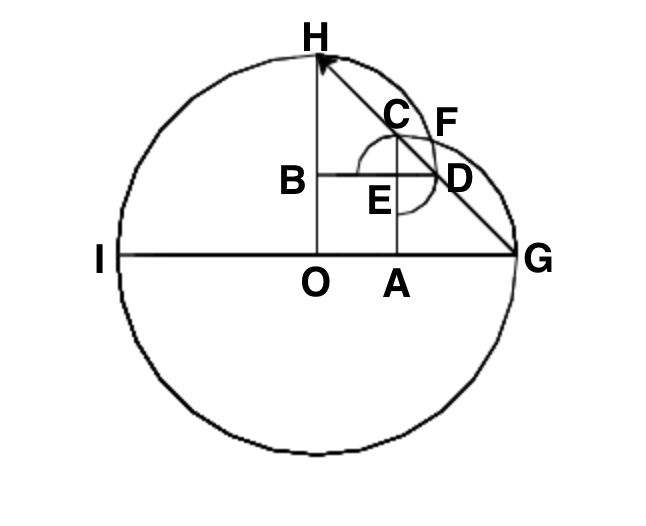
\includegraphics{grazing-area-challenge-exercise-2-quanta-rotated}
\centering
\end{figure}

Note that the goat is tied at $O$.

To find the area that the goat can graze in, you would have to add the area of the region $GIH$ (which is three quarters of a circle of radius 10 units), the area of the region $BDFH$ (which is a quarter of a circle of radius 6 units) and the area of the region $AGFC$ (which is a quarter of a circle of radius 6 units). Then you have to subtract the area of the region $EDFC$.

The main challenge here is to calculate the area of the region $EDFC$.

First, note that arcs $CF$ and $DF$ are of equal length. To see this, join $A$ and $B$, $B$ and $F$, and $A$ and $F$. Then, in $\triangle ABF$, $AF = BF$ because $AF = AC$ (since they are the radii of the same circle) and $BF = BD$ (again, since they are the radii of the same circle) and $AC = BD =$ 6 units. Therefore, $\angle ABF = \angle BAF$. But since $\angle ABE = \angle BAE = 45^\circ$, therefore $\angle DBF = \angle EBF = \angle ABF - \angle ABE = \angle BAF - \angle BAE = \angle EAF = \angle CAF$. Now, since the radii and the angles of the arcs $CF$ and $DF$ are equal, so the two arcs are of equal length.

Now, to find the area of the region $EDFC$, we'll use calculus. Here's the approach we'll use. We'll draw a line $FJ$ perpendicular to $OG$. This line will intersect $OG$ at $J$ and $BD$ at $K$. Similarly, we'll draw a line $FL$ perpendicular to $OH$. This line will intersect $OH$ at $L$ and $AC$ at $M$. Now, we'll use integration to calculate the areas of the regions $FKD$ and $FMC$. The sum of these two areas and the area of the rectangle $EKFM$ would give us the area of the region $EDFC$.

To start with, we'll have a coordinate system with the origin at $O$, $OG$ as the $X$-axis and $OH$ as the $Y$-axis. Also, draw $DP$ perpendicular to $OG$. Here, $P$ is the point of intersection between $DP$ and $OG$. Similarly, draw $CQ$ perpendicular to $OH$, where $Q$ is the point of intersection of $CQ$ with $OH$.

Now, let's find the coordinates of the point $F$. Note that the point $F$ is the intersection of the arcs of the circles with equations $(x - 4)^2 + y^2 = 6^2$ and $x^2 + (y - 4)^2 = 6^2$. If you expand the two equations, you'll get $x^2 - 8x + 16 + y^2 = 36$ and $x^2 + y^2 - 8y + 16 = 36$. Now, if you subtract the first equation from the second, you'll get $8x - 8y = 0$ or $x = y$. Substituting this in either equation, you'll get $2x^2 - 8x + 16 = 36$. Simplifying, you'll get $x^2 - 4x - 10 = 0$. This can be solved to get $x = y = \frac{4 \pm \sqrt{16 + 40}}{2} = 2 \pm \sqrt{14}$. Since we're only interested in values in the first quadrant, we'll take $x = y = 2 + \sqrt{14}$. So, the coordinates of $F$ are $(2 + \sqrt{14}, 2 + \sqrt{14})$.
\\
\par
$\begin{aligned}
\text{Now, area of } FJPD & = \int_{2 + \sqrt{14}}^6 4 + \sqrt{36 - x^2} \, dx \\
& = \int_{2 + \sqrt{14}}^6 4 \, dx + \int_{2 + \sqrt{14}}^6 \sqrt{36 - x^2} \, dx \\
& = 4x \, \biggr\rvert_{2 + \sqrt{14}}^6 + \frac{6^2}{2}\Biggl(\frac{x \sqrt{6^2 - x^2}}{6^2} - \cos^{-1} \frac{x}{6} \Biggr) \, \biggr\rvert_{2 + \sqrt{14}}^6 \\
& = 4 (6 - 2 - \sqrt{14}) + 18 \Biggl( 0 - \frac{(2 + \sqrt{14}) \sqrt{6^2 - (2 + \sqrt{14})^2}}{36} + \cos^{-1} \frac{2 + \sqrt{14}}{6} \Biggr) \\
& \approx 1.335
\end{aligned}$
\\
\par
Note that the integral $\int \sqrt{36 - x^2} \, dx$ that appears above is of the form $\int \sqrt{a^2 - x^2} \, dx$ which can be easily computed by using the substitution $x = a \cos \theta$. Also, $\sqrt{6^2 - (2 + \sqrt{14})^2}$ can be simplified to $\sqrt{14} - 2$.

Now, you can get the area of the region $FKD$ by subtracting the area of the rectangle $KJPD$ (which is equal to $4(6 - (2 + \sqrt{14})) \approx 1.033$ square units) from the area of $FJPD$.
\\
\par
$\begin{aligned}
\text{Similarly, area of } CAJF & = \int_4^{2 + \sqrt{14}} \sqrt{36 - (x - 4)^2} \, dx \\
& = \frac{6^2}{2} \Biggl( \frac{(x - 4) \sqrt{6^2 - (x - 4)^2}}{6^2} - \cos^{-1} \frac{x - 4}{6} \Biggr) \biggr\rvert_4^{2 + \sqrt{14}} \\
& \approx 10.301
\end{aligned}$
\\
\par
The above integral can be computed by transforming it to an integral of the from $\int \sqrt{a^2 - x^2} \, dx$ by using the substitution $X = x - 4$.

Now, the area of the region $FMC$ can be computed by subtracting the area of the rectangle $MAJF$ (which is equal to $(2 + \sqrt{14})(2 + \sqrt{14} - 4) = 14 - 4 = 10$ square units) from the area of $CAJF$.

\end{document}
